\documentclass[10pt]{beamer}

\setbeamertemplate{note page}[default]
\setbeameroption{hide notes}
%\setbeameroption{show only notes}
%\setbeameroption{show notes}


\usetheme[progressbar=frametitle]{metropolis}
\usepackage{appendixnumberbeamer}

\usepackage{booktabs}
\usepackage[scale=2]{ccicons}

\usepackage{pgfplots}
\usepgfplotslibrary{dateplot}
\usepackage{multicol}
\setlength{\columnsep}{1.5cm}

\usepackage{animate}
\usepackage{lmodern}
\usepackage[T1]{fontenc}
\usepackage{mathtools}
\usepackage{graphicx}
\usepackage{caption}

\definecolor{set1}{RGB}{228, 26, 28}
\definecolor{set2}{RGB}{77, 175, 74}
\definecolor{set3}{RGB}{255, 127, 0}
\definecolor{set4}{RGB}{166, 86, 40}
\definecolor{set5}{RGB}{153, 153, 153}

\usepackage{xspace}
\newcommand{\themename}{\textbf{\textsc{metropolis}}\xspace}

\newcommand\Fontvi{\fontsize{8}{9}\selectfont}
\newcommand\Fontvr{\fontsize{6}{7}\selectfont}

\setbeamerfont{parent A}{size=\small}


\title{Digital Transformation of Healthcare}
\subtitle{Building a Data Driven Pipeline}
% \date{\today}
\date{}
\author{Michoel Snow, M.D. Ph.D., Glen Ferguson, Ph.D.}
\institute{Center for Health Data Innovations}
% \titlegraphic{\hfill\includegraphics[height=1.5cm]{logo.pdf}}

\begin{document}

\maketitle


\begin{frame}{Digital Transformation of Healthcare}
	\begin{itemize}
		\item Healthcare Informatics
		\begin{itemize}
			\item The management and use of patient healthcare information driven by insights gained using health information technology
			\item The goal is to provide higher quality care (lower cost, greater availability, new healthcare opportunities) to our patients
		\end{itemize}
		\item Course Objectives
		\begin{itemize}
			\item Outline the components which form model bioinformatics pipelines
			\item Investigate possible hypotheses for clinical significance and system compliance
			\item Characterize hypotheses within the context of healthcare infrastructure 
			\item Identify stakeholders based on the scope of the project
			\item Identify sources of patient data and differentiate the various collection mechanisms/tools
			\item Develop a informatics driven research question
			\item Assess the quality of the generated data 
			\item Describe modeling frameworks to analyze the data 
			\item Contrast methods to evaluate the results of modeling
			\item Discuss methods of model implementation and care provider communication
			\item Design new bioinformatics pipeline for application within the healthcare system
		\end{itemize}
	\end{itemize}
\end{frame}


\begin{frame}{Course Overview}
	\begin{itemize}
		\item Lecture format 
		\begin{itemize}
			\item Each class will focus on a specific part of the pipeline
			\item Explore theoretical constructs through discussion and small group work
			\item Work through real world cases using theoretical framework
		\end{itemize}	
		\item Final Project
		\begin{itemize}
			\item Each student will present an informatics project to the class over the last two lectures
		\end{itemize}
		\item Grading
		\begin{itemize}
			\item Class is Pass/Fail
			\item Grade is based on participation and final project 
		\end{itemize}		
		\item Course Leaders
		\begin{itemize}
			\item Michoel Snow - msnow1@montefiore.org
			\item Glen Ferguson - glfergus@montefiore.org
		\end{itemize}
	\end{itemize}
\end{frame}



\begin{frame}{Lecture Schedule}
	\begin{enumerate}
		\small
		\item Overview of course and introduction to building data driven bioinformatic pipelines
		\item Building clinical decision support systems (Implementation)
		\item Evaluating study results and model predictions (Modeling and Analysis) 
		\item Overview of machine learning models - part 1 (Modeling and Analysis)
		\item Overview of machine learning models - part 2 (Modeling and Analysis)
		\item Assessing data quality and preparing data for modeling and analysis (Data Preparation)
		\item Identifying data sources and implementing collection protocols (Data Collection)
		\item Calculating economic feasability and impact (Stakeholder concerns)
		\item Bioinformatics ethics and stakeholder engagement (Stakeholder Concerns)
		\item Healthcare administrative databases (Infrastructure)
		\item Exploratory data analysis (Hypothesis Generation)
		\item Presentations - part 1
		\item Presentations - part 2
	\end{enumerate}
\end{frame}

\begin{frame}{Any Questions}
	\begin{center}
		\Huge ?	
	\end{center}
\end{frame}



\begin{frame}{Objectives}
	After this lecture students will be able to 
	\begin{itemize}
		\item Describe the different phases of a healthcare informatics project 
		\item Diagram an informatics project as a pipeline
	\end{itemize}
\end{frame}


% 30 minutes
\begin{frame}{Metastatic Epidural Spinal Cord Compression}
	\begin{itemize} % Draw the 5 stages and 8 boxes of the healthcare informatics pipeline
		\item Overview
		\begin{itemize}
			\item Occurs in 2\% to 5\% of all cancer patients
			\item Cord compression is the first manifestation in about 20\% of patients
			\item Survival is generally less than 6 months
			\item Prognosis negatively correlates with severity of presenting symptoms
		\end{itemize}
		\item Diagnosis
		\begin{itemize}
			\item Clinical Findings + Imaging (MRI or CT)
		\end{itemize}
		\item Treatment
		\begin{itemize}
			\item Surgery
			\item Radiation therapy
		\end{itemize}
	\end{itemize}
%	\pause[2]
	\begin{center}
		\only<2>{\Large Let's build our own pipeline for spinal cord compression}
	\end{center}
\end{frame}


\note{
\begin{itemize}
	\item First let's talk about the 4 to 5 basic steps in our pipeline, and then we'll break each step down into 1 to 3 sub-steps, and then discuss the components of the individual sub-steps.  The first two parts we'll do together as a group and the last part you will work on in teams
%	\item  \textbf{Conceptiation} Meaningful question (Prediction vs detection), significant hypothesis (can detect earlier, can predict months ahead of time using imaging)
%	\item \textbf{Initiation - infrastructure} 
\end{itemize}
}




\begin{frame}{Healthcare Informatics Pipeline}
	\begin{center}
		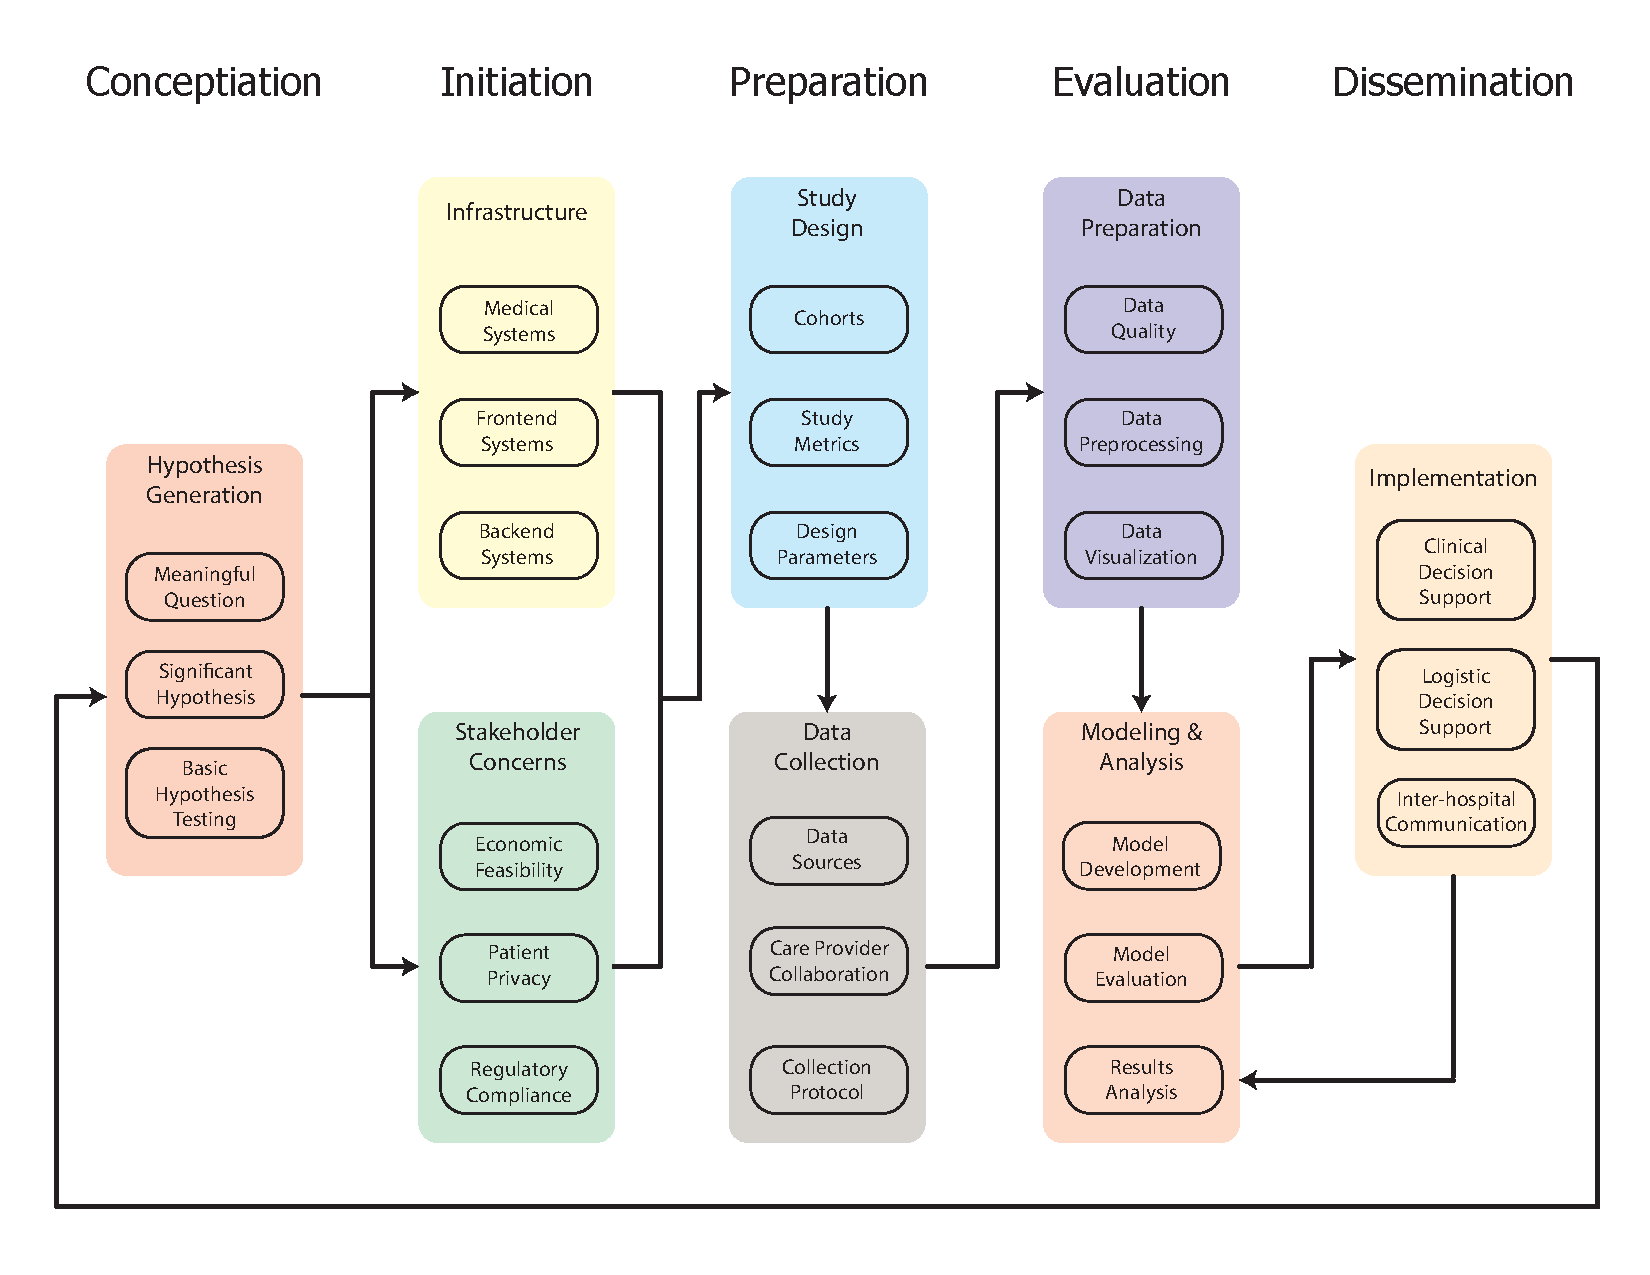
\includegraphics[width=0.9\textwidth]{images/informatics_pipeline.pdf}	
	\end{center}
\end{frame}


\begin{frame}{Further Reading}
	\begin{itemize}
		\item Weapons of Math Destruction
		\item Journal of the American Medical Informatics Association (JAMIA)
		\item Journal of Internet Medical Research
		\item arXiv.org
	\end{itemize}
\end{frame}





%\begin{frame}{Metastatic Epidural Spinal Cord Compression}
%Initial Steps
%	\begin{itemize} % Draw the 5 stages and 8 boxes of the healthcare informatics pipeline
%		\item Question
%		\begin{itemize}
%			\item Question
%			\item Cord Compression is the first manifestation in about 20\% of patients
%			\item Survival is generally less than 6 months
%			\item Prognosis negatively correlates with severity of presenting symptoms
%		\end{itemize}
%		\item Exploratory Analysis
%		\begin{itemize}
%			\item Clinical Findings
%			\item Imaging (MRI or CT)
%		\end{itemize}
%	\end{itemize}
%\end{frame}


\end{document}